\begin{titlepage}
\begin{center}

% Upper part of the page. The '~' is needed because only works if a paragraph has started.

\includegraphics[width=0.35\textwidth]{./Logo_Polytech_Sorbonne}~\\[1cm]

\textsc{\LARGE Polytech Sorbonne}\\[1.5cm]

\textsc{\Large }\\[0.5cm]

% Title
\HRule \\[0.4cm]

{\huge \bfseries Projet\\
Analyse numérique d’instruments à cordes \\[0.4cm] }

\HRule \\[1.5cm]

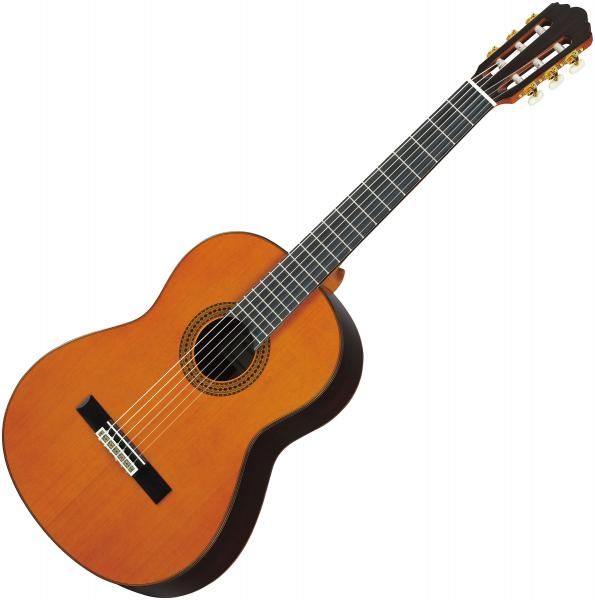
\includegraphics[width=0.35\textwidth]{./guitare}~\\[1cm]

% Author and supervisor
\begin{minipage}{0.4\textwidth}
\begin{flushleft} \large
BENELKATER \textsc{Mohamed}\\
BURBANO \textsc{Paula}\\
COMBARET \textsc{Léo}\\
FIDA CYRILLE \textsc{Rudio}\\
PREVOT \textsc{Alexia}\\
RAKOTOVAO \textsc{Jonathan}
\end{flushleft}
\end{minipage}
\begin{minipage}{0.4\textwidth}
\begin{flushright} \large
\emph{Encadrant:} \\
Yann \textsc{TEYTAUT}\\
\emph{MAIN3} \\
2020/2021
\end{flushright}
\end{minipage}

\vfill

% Bottom of the page
{\large \today}

\end{center}
\end{titlepage}